We propose a flexible data processing and analysis framework based entirely on open-source projects, which can run on local machines, small clusters or even cloud computing platforms, such as Amazon Web Services. 

\subsection{Architecture}
To create and manage independent processing infrastructure we propose to use Docker containers. This enables the application to run on different machines with different operating systems having Docker and Compose installed as the only requirement. 

The containers are started by Docker Compose. There is a driver container that launches Jupyter notebooks on \url{http://localhost:8888} and can run python notebooks with pynb. 
Jupyter notebook is an open-source tool for data science, that allows the users to execute scripts in an interactive fashion. It supports different programming languages and frameworks such as Python, R, pySpark and so on. It is mostly used for prototyping, since it is not suitable for clean and sustainable code with proper version control. Also it is not possible to automate running Jupyter notebooks as tasks. 
Pynb is a tool that allows to convert Jupyter notebooks to plain python code and vice verse. The maintenance of such python notebooks is more sustainable and it is possible to programatically run them. \cite{pynb}

The driver runs pySpark applications on the standalone Spark cluster with one or more workers and one master with client deploy mode. In standalone cluster mode, Spark's own cluster manager is used instead of YARN or Mesos. Client deploy mode means that  the driver is launched in the same process as the client that submits the application. 

A master container that deploys Spark master, and one or more worker containers that starts the workers with specified cores and memory, connected to the master. The Spark web user interface shows the available worker on \url{http://localhost:8080}.

As a data-source we suggest Parquet over .csv, since most of the operations in the project involve iterating through all rows for given columns. This way we take advantage of the Parquet being an efficient columnar storage.

In Python the DataSet API is not available, but the Data-frame API is. DataFrames have a rich library of functions including string manipulation, date arithmetic, common math operations and they provide a similar interface to DataFrames in Python's Pandas library or to relational tables. \cite{spark-sql}

Internally, Spark SQL has information about the structure of both the data and the computation to perform extra optimizations. 

One of the great advantages of using Spark DataFrames is that they come with built-in optimizations as opposed to RDDs where the developer has to design the transformations and operations in way that the execution is optimal.

Another advantage is that Spark DataFrames can be quickly and seamlessly constructed from a different sources such as: structured data files, tables in Hive, external databases, or existing RDDs. The DataFrame API is available in Scala, Java, Python, and R. DataFrame operations are referred as "untyped transformations" in contrast to "typed transformations" executed on Datasets.\cite{spark-sql} 

The most common operators in this analysis were filtering, joining, counting and sorting the DataFrames.

Fabric can be used to orchestrate the containers, run tests and execute tasks. It is more convenient to use a unified command line interface for recurring administration tasks. \cite{fabric}

\subsection{Data processing}\label{sec:data-proc}
The data-flow throughout the implementation steps can be seen on Figure \ref{fig:data-flow}.
\begin{figure}[h]
    \centering
    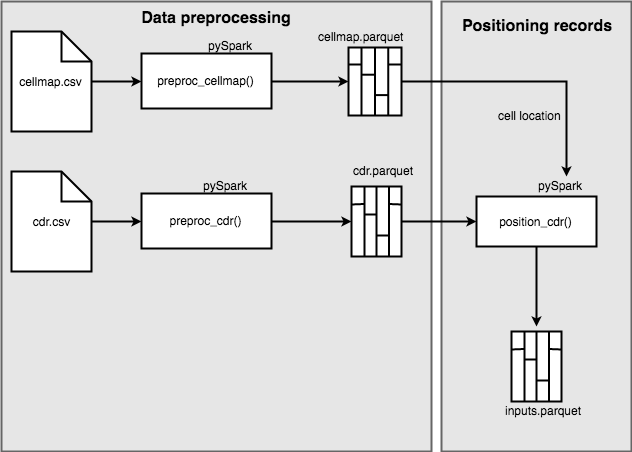
\includegraphics[width=0.5\textwidth]{images/data-flow.png}
    \caption{Data flow}
    \label{fig:data-flow}
\end{figure}

We prpose processing the data in PySpark DataFrames as the Pandas data frames cannot handle the size of the data sets. After pre-processing the data it is recommended to store them in Parquet files instead of .csv files.

\subsection{Trajectory distance calculation}
As the users tend to move while using their phones, the generated CDR observations have semantics of trajectories. CDR data points can be grouped as trajectories so that the characteristics of trajectories and the result of previous research already conducted in this field can be utilized for achieving more accurate positioning.

We compare the ground truth GPS trajectories to trajectories of CDR events for the same time window as shown in Figure \ref{fig:problem}. 
\begin{figure}[h]
    \centering
    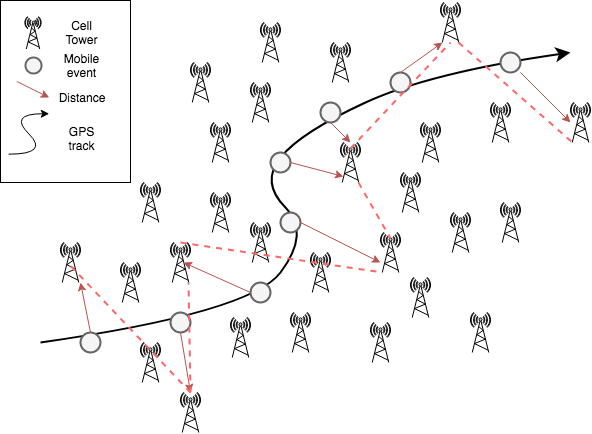
\includegraphics[width=0.45\textwidth]{images/problem.png}
    \caption{Schematic illustration of the research problem}
    \label{fig:problem}
\end{figure}

To evaluate cellular network event based customer localization we calculate the Euclidean distance and the edit distance along with several statistics of the pairwise distances between ground truth GPS trajectories and mobile network event trajectories. The Haversine distance is used to define the spatial distance between points. In the mobile network event trajectory, the location information is obtained from cell map data set.

Similarly to the formulation in \cite{encyclopedia} and \cite{distance-def} we define distance measure on trajectories, such as:
\begin{definition}
Let $\mathcal{M}$ be a set of trajectories. A function $D :\mathcal{M} \times \mathcal{M} \rightarrow \mathcal{R}$ \nomenclature{$D$}{Distance measure defined on a set of trajectories.} is called a dissimilarity (distance) on $\mathcal{M}$ if for all $T_{1}, T_{2} \in \mathcal{M}$: 
\begin{itemize}
    \item $D(T_{1},T_{2}) \geqslant 0$
    \item $D(T_{1},T_{2}) = d(T_{2},T_{2})$
    \item $D(T_{1},T_{1}) = 0$
\end{itemize}
If all of these conditions are satisfied and $D(T_{1}, T_{2}) = 0 \Rightarrow  T_{1} = T_{2} $ is considered to be a symmetric. If
the triangle inequality is also satisfied, $D$ is a metric.
\end{definition}

The \textit{Euclidean distance} (or inverse similarity) measure between two trajectories is used in this analysis:
\[D(T,\Tilde{T}) = \sqrt{\sum_{i=1}^{n} (d(P_{i},\Tilde{P_{i}}))^{2}}\]

where $d((P_{i},\Tilde{P_{i}})$ refers to the spatial distance between two points given with the Haversine formula.

The Euclidean distance algorithm presented in Algorithm \ref{algo:euclidean} is implemented with Pandas UDFs invoked on PySpark data frames. Pandas UDFs convert the columns of Spark data frames into Pandas Series and they also return Pandas Series, which eliminates row by row iteration in contrast with standard UDFs in PySpark.

\begin{algorithm}
\begin{algorithmic}
\caption{Euclidean distance function on trajectories} \label{algo:euclidean}
\Function{euclideanDist}{Traj tReal, Traj tApprox}
\State dEuclidean = 0
\State nPoints = len(tReal) 
\For{i \textbf{in} 0 to nPoints}
    \State dEuclidean = dEuclidean + power(haversine(     
    \State tReal[i], tApprox[i]) , 2)
\EndFor
\Return sqrt(dEuclidean)
\EndFunction
\end{algorithmic}
\end{algorithm}


